\section{main.h File Reference}
\label{main_8h}\index{main.h@{main.h}}
{\tt \#include $<$stdio.h$>$}\par
{\tt \#include $<$QApplication$>$}\par
{\tt \#include $<$QClipboard$>$}\par
{\tt \#include $<$QObject$>$}\par
{\tt \#include $<$QWidget$>$}\par
{\tt \#include $<$QDialog$>$}\par
{\tt \#include $<$Qt\-Global$>$}\par
{\tt \#include $<$QDom\-Node$>$}\par
{\tt \#include $<$QTree\-View$>$}\par
{\tt \#include $<$QText\-Edit$>$}\par
{\tt \#include $<$QPush\-Button$>$}\par
{\tt \#include $<$QVBox\-Layout$>$}\par
{\tt \#include $<$QSize\-Policy$>$}\par
{\tt \#include \char`\"{}mainwindow.h\char`\"{}}\par


Include dependency graph for main.h:\begin{figure}[H]
\begin{center}
\leavevmode
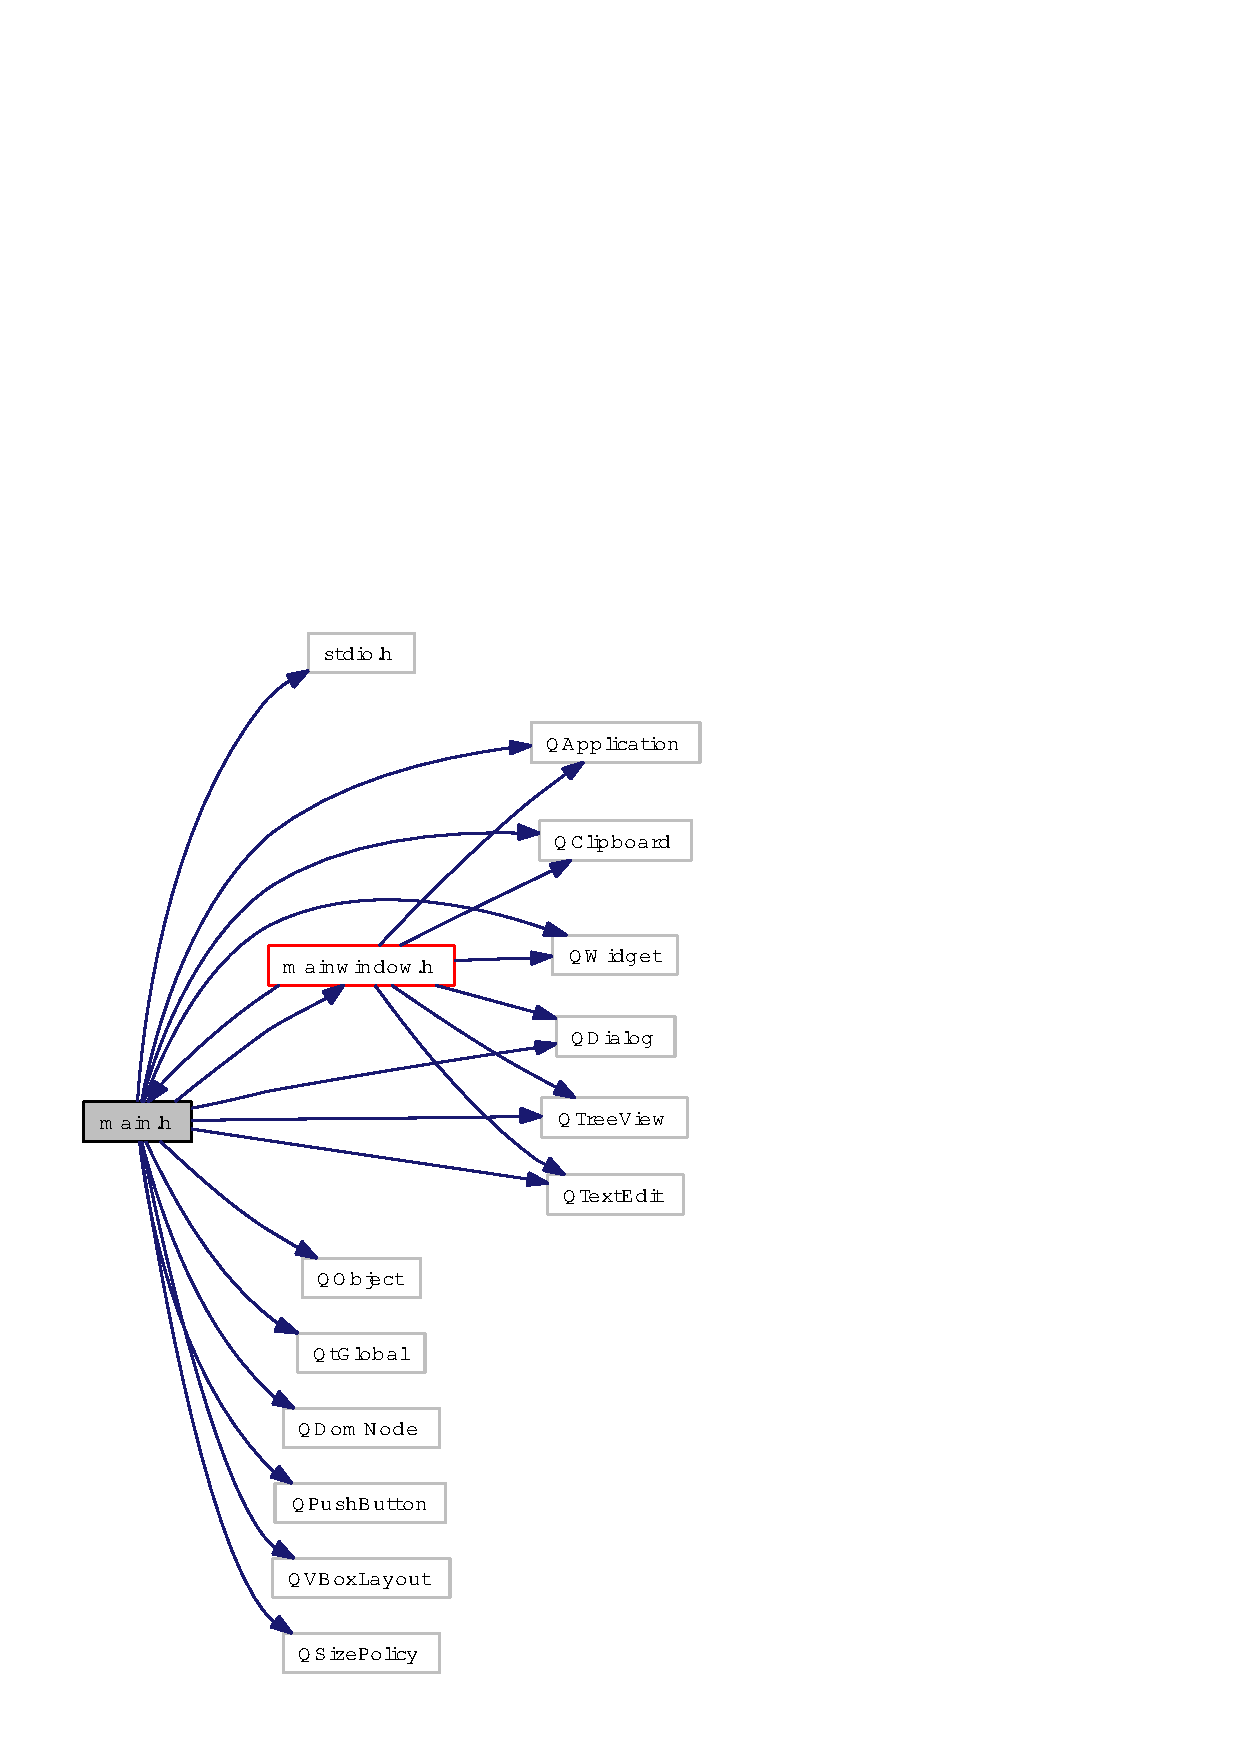
\includegraphics[width=170pt]{main_8h__incl}
\end{center}
\end{figure}


This graph shows which files directly or indirectly include this file:\begin{figure}[H]
\begin{center}
\leavevmode
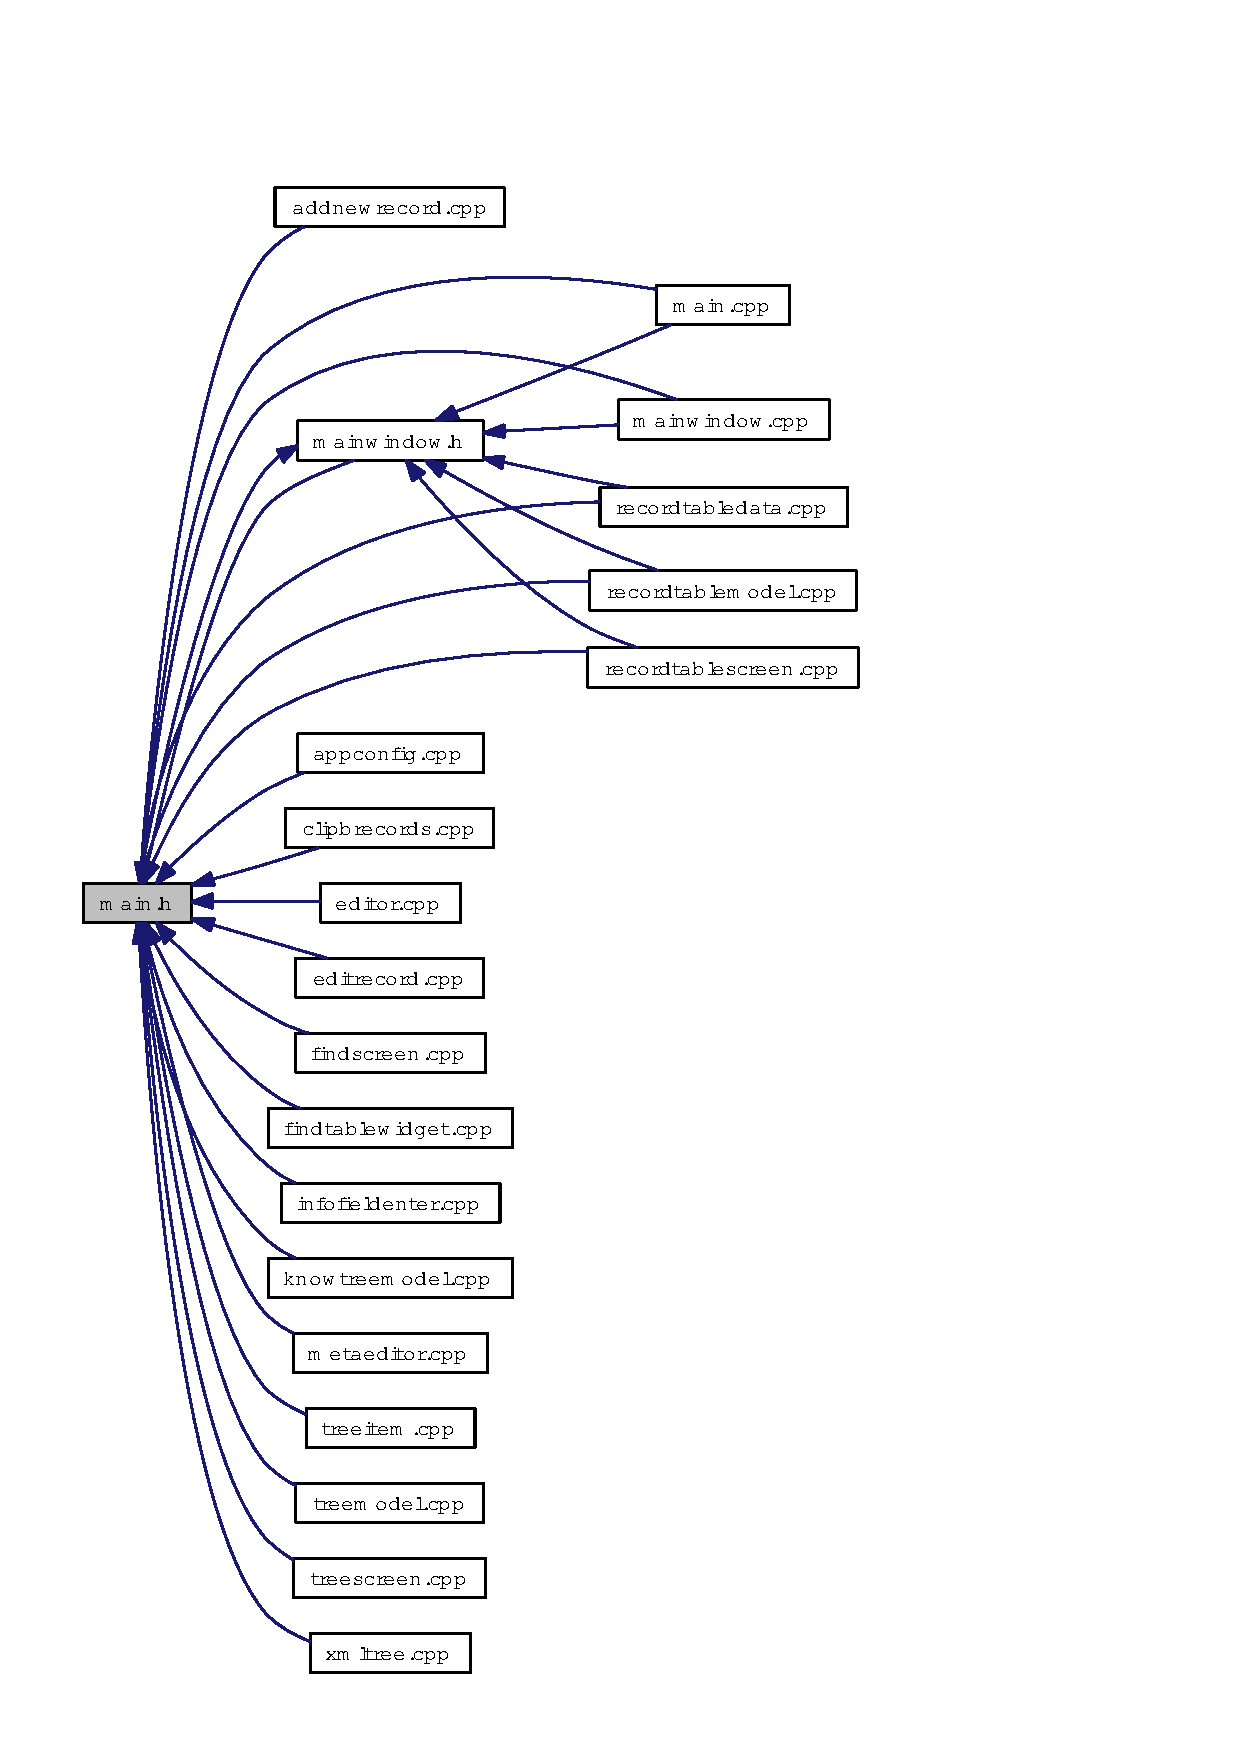
\includegraphics[width=208pt]{main_8h__dep__incl}
\end{center}
\end{figure}
\subsection*{Defines}
\begin{CompactItemize}
\item 
\#define {\bf GAME\_\-RELEASE\_\-VERSION}~0
\item 
\#define {\bf GAME\_\-RELEASE}~114
\item 
\#define {\bf COMPILE\_\-MODE}~0
\item 
\#define {\bf DEBUG\_\-PRINT}
\item 
\#define {\bf CURRENT\_\-FORMAT\_\-VERSION}~1
\item 
\#define {\bf CURRENT\_\-FORMAT\_\-SUBVERSION}~1
\item 
\#define {\bf DPF}(X)~logprint X
\end{CompactItemize}
\subsection*{Functions}
\begin{CompactItemize}
\item 
void {\bf logprint} (char $\ast$lpsz\-Text,...)
\item 
void {\bf critical\_\-error} (QString message)
\item 
void {\bf info\_\-window} (QString i)
\item 
QString {\bf xmlnode\_\-to\_\-string} (QDom\-Node xmldata)
\item 
QString {\bf convert\_\-to\_\-lastnumformat} (int n)
\item 
void {\bf remove\_\-dir} (QString namedirfrom)
\item 
void {\bf print\_\-object\_\-tree} (void)
\item 
bool {\bf compare\_\-QString\-List\_\-len} (const QString\-List \&list1, const QString\-List \&list2)
\item 
int {\bf imax} (int x1, int x2)
\item 
int {\bf imin} (int x1, int x2)
\item 
template$<$class X$>$ X $\ast$ {\bf find\_\-object} (QString n)
\end{CompactItemize}


\subsection{Define Documentation}
\index{main.h@{main.h}!COMPILE_MODE@{COMPILE\_\-MODE}}
\index{COMPILE_MODE@{COMPILE\_\-MODE}!main.h@{main.h}}
\subsubsection{\setlength{\rightskip}{0pt plus 5cm}\#define COMPILE\_\-MODE~0}\label{main_8h_2c268a5f82ee3a6df7fd780174bdffcb}




Definition at line 73 of file main.h.\index{main.h@{main.h}!CURRENT_FORMAT_SUBVERSION@{CURRENT\_\-FORMAT\_\-SUBVERSION}}
\index{CURRENT_FORMAT_SUBVERSION@{CURRENT\_\-FORMAT\_\-SUBVERSION}!main.h@{main.h}}
\subsubsection{\setlength{\rightskip}{0pt plus 5cm}\#define CURRENT\_\-FORMAT\_\-SUBVERSION~1}\label{main_8h_c0afd906320d22ab872498bfd98b2bb9}




Definition at line 87 of file main.h.

Referenced by treescreen::save\_\-knowtree().\index{main.h@{main.h}!CURRENT_FORMAT_VERSION@{CURRENT\_\-FORMAT\_\-VERSION}}
\index{CURRENT_FORMAT_VERSION@{CURRENT\_\-FORMAT\_\-VERSION}!main.h@{main.h}}
\subsubsection{\setlength{\rightskip}{0pt plus 5cm}\#define CURRENT\_\-FORMAT\_\-VERSION~1}\label{main_8h_13494493ae4a0f9ce61e04759b1666b4}




Definition at line 86 of file main.h.

Referenced by treescreen::save\_\-knowtree().\index{main.h@{main.h}!DEBUG_PRINT@{DEBUG\_\-PRINT}}
\index{DEBUG_PRINT@{DEBUG\_\-PRINT}!main.h@{main.h}}
\subsubsection{\setlength{\rightskip}{0pt plus 5cm}\#define DEBUG\_\-PRINT}\label{main_8h_d5aeca1a1a793c8ba18f85cbac89e768}




Definition at line 79 of file main.h.\index{main.h@{main.h}!DPF@{DPF}}
\index{DPF@{DPF}!main.h@{main.h}}
\subsubsection{\setlength{\rightskip}{0pt plus 5cm}\#define DPF(X)~logprint X}\label{main_8h_ae074830d7dd3260e034d3acb8479e92}




Definition at line 91 of file main.h.

Referenced by main().\index{main.h@{main.h}!GAME_RELEASE@{GAME\_\-RELEASE}}
\index{GAME_RELEASE@{GAME\_\-RELEASE}!main.h@{main.h}}
\subsubsection{\setlength{\rightskip}{0pt plus 5cm}\#define GAME\_\-RELEASE~114}\label{main_8h_6b7b35a1e0fcf283c8f8ff89cf8bdf4f}




Definition at line 68 of file main.h.

Referenced by main().\index{main.h@{main.h}!GAME_RELEASE_VERSION@{GAME\_\-RELEASE\_\-VERSION}}
\index{GAME_RELEASE_VERSION@{GAME\_\-RELEASE\_\-VERSION}!main.h@{main.h}}
\subsubsection{\setlength{\rightskip}{0pt plus 5cm}\#define GAME\_\-RELEASE\_\-VERSION~0}\label{main_8h_94dfb3fd9ca31fbe7086f0c28b1257d7}




Definition at line 67 of file main.h.

Referenced by main().

\subsection{Function Documentation}
\index{main.h@{main.h}!compare_QStringList_len@{compare\_\-QStringList\_\-len}}
\index{compare_QStringList_len@{compare\_\-QStringList\_\-len}!main.h@{main.h}}
\subsubsection{\setlength{\rightskip}{0pt plus 5cm}bool compare\_\-QString\-List\_\-len (const QString\-List \& {\em list1}, const QString\-List \& {\em list2})}\label{main_8h_4b9267e7db7804b40590ebb0aae4c257}




Definition at line 223 of file main.cpp.\index{main.h@{main.h}!convert_to_lastnumformat@{convert\_\-to\_\-lastnumformat}}
\index{convert_to_lastnumformat@{convert\_\-to\_\-lastnumformat}!main.h@{main.h}}
\subsubsection{\setlength{\rightskip}{0pt plus 5cm}QString convert\_\-to\_\-lastnumformat (int {\em n})}\label{main_8h_ec163ac31ec8c8183dc05762ecb4281d}




Definition at line 107 of file main.cpp.\index{main.h@{main.h}!critical_error@{critical\_\-error}}
\index{critical_error@{critical\_\-error}!main.h@{main.h}}
\subsubsection{\setlength{\rightskip}{0pt plus 5cm}void critical\_\-error (QString {\em message})}\label{main_8h_fe5e42a76086b3d9d2912f0c17ef0e59}




Definition at line 42 of file main.cpp.

Referenced by appconfig::appconfig(), Tree\-Item::data(), editrecord::get\_\-field(), infofieldenter::get\_\-field(), recordtabledata::get\_\-field(), recordtabledata::get\_\-fields(), appconfig::get\_\-parameter(), clipbrecords::get\_\-record(), recordtabledata::get\_\-text(), Tree\-Model::get\-Item(), recordtabledata::insert\_\-new\_\-record(), recordtablescreen::select(), appconfig::set\_\-addnewrecord\_\-expand\_\-info(), editrecord::set\_\-field(), infofieldenter::set\_\-field(), metaeditor::set\_\-field(), and recordtabledata::set\_\-field().

Here is the caller graph for this function:\begin{figure}[H]
\begin{center}
\leavevmode
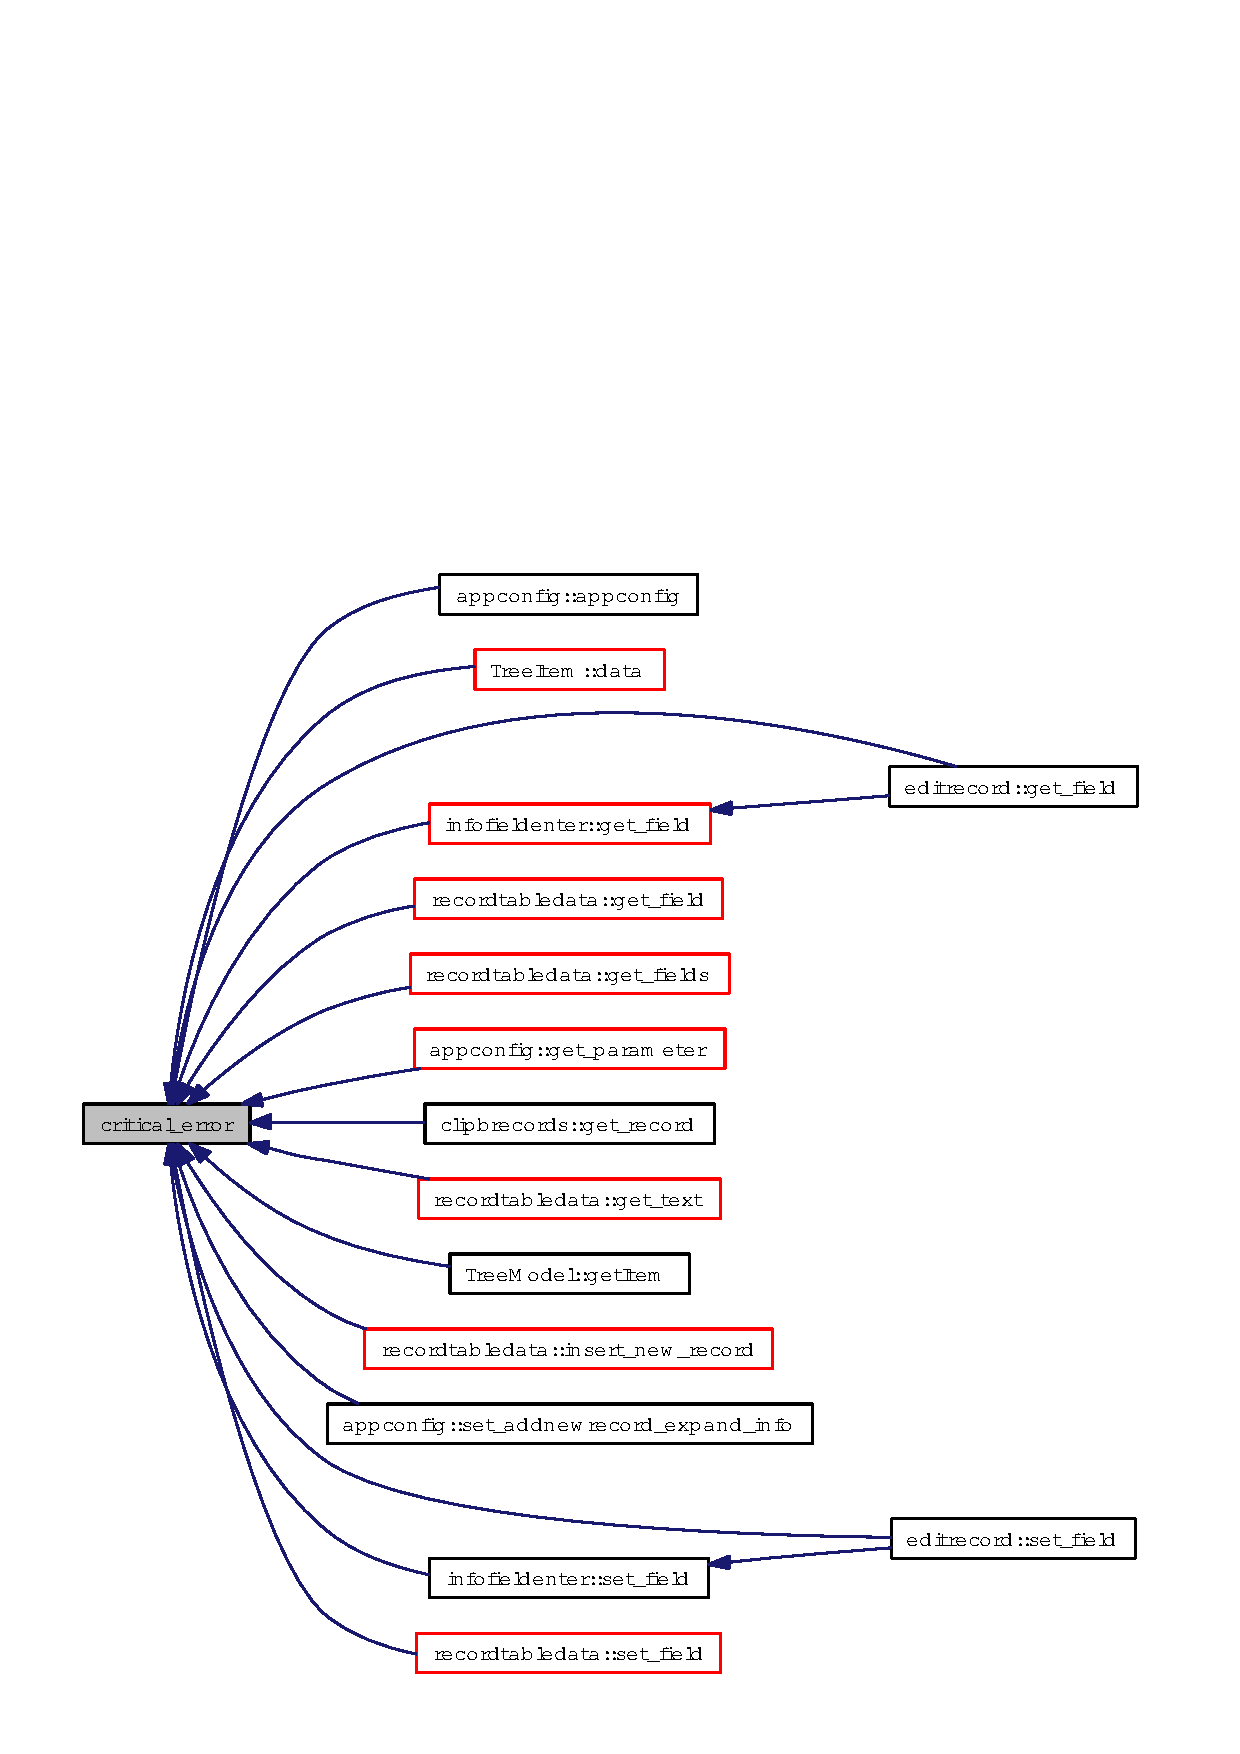
\includegraphics[width=275pt]{main_8h_fe5e42a76086b3d9d2912f0c17ef0e59_icgraph}
\end{center}
\end{figure}
\index{main.h@{main.h}!find_object@{find\_\-object}}
\index{find_object@{find\_\-object}!main.h@{main.h}}
\subsubsection{\setlength{\rightskip}{0pt plus 5cm}template$<$class X$>$ X$\ast$ find\_\-object (QString {\em n})\hspace{0.3cm}{\tt  [inline]}}\label{main_8h_cf7faff64ef33261f53a1cb145cc92c3}




Definition at line 112 of file main.h.

References mainwindowpointer.\index{main.h@{main.h}!imax@{imax}}
\index{imax@{imax}!main.h@{main.h}}
\subsubsection{\setlength{\rightskip}{0pt plus 5cm}int imax (int {\em x1}, int {\em x2})}\label{main_8h_99d8888037c7927cbe6362f80a2f6f8b}




Definition at line 229 of file main.cpp.\index{main.h@{main.h}!imin@{imin}}
\index{imin@{imin}!main.h@{main.h}}
\subsubsection{\setlength{\rightskip}{0pt plus 5cm}int imin (int {\em x1}, int {\em x2})}\label{main_8h_6c9ac00d126f1109a583b5264a07412a}




Definition at line 236 of file main.cpp.

Referenced by findscreen::setup\_\-toolsline(), and infofieldenter::setup\_\-ui().

Here is the caller graph for this function:\begin{figure}[H]
\begin{center}
\leavevmode
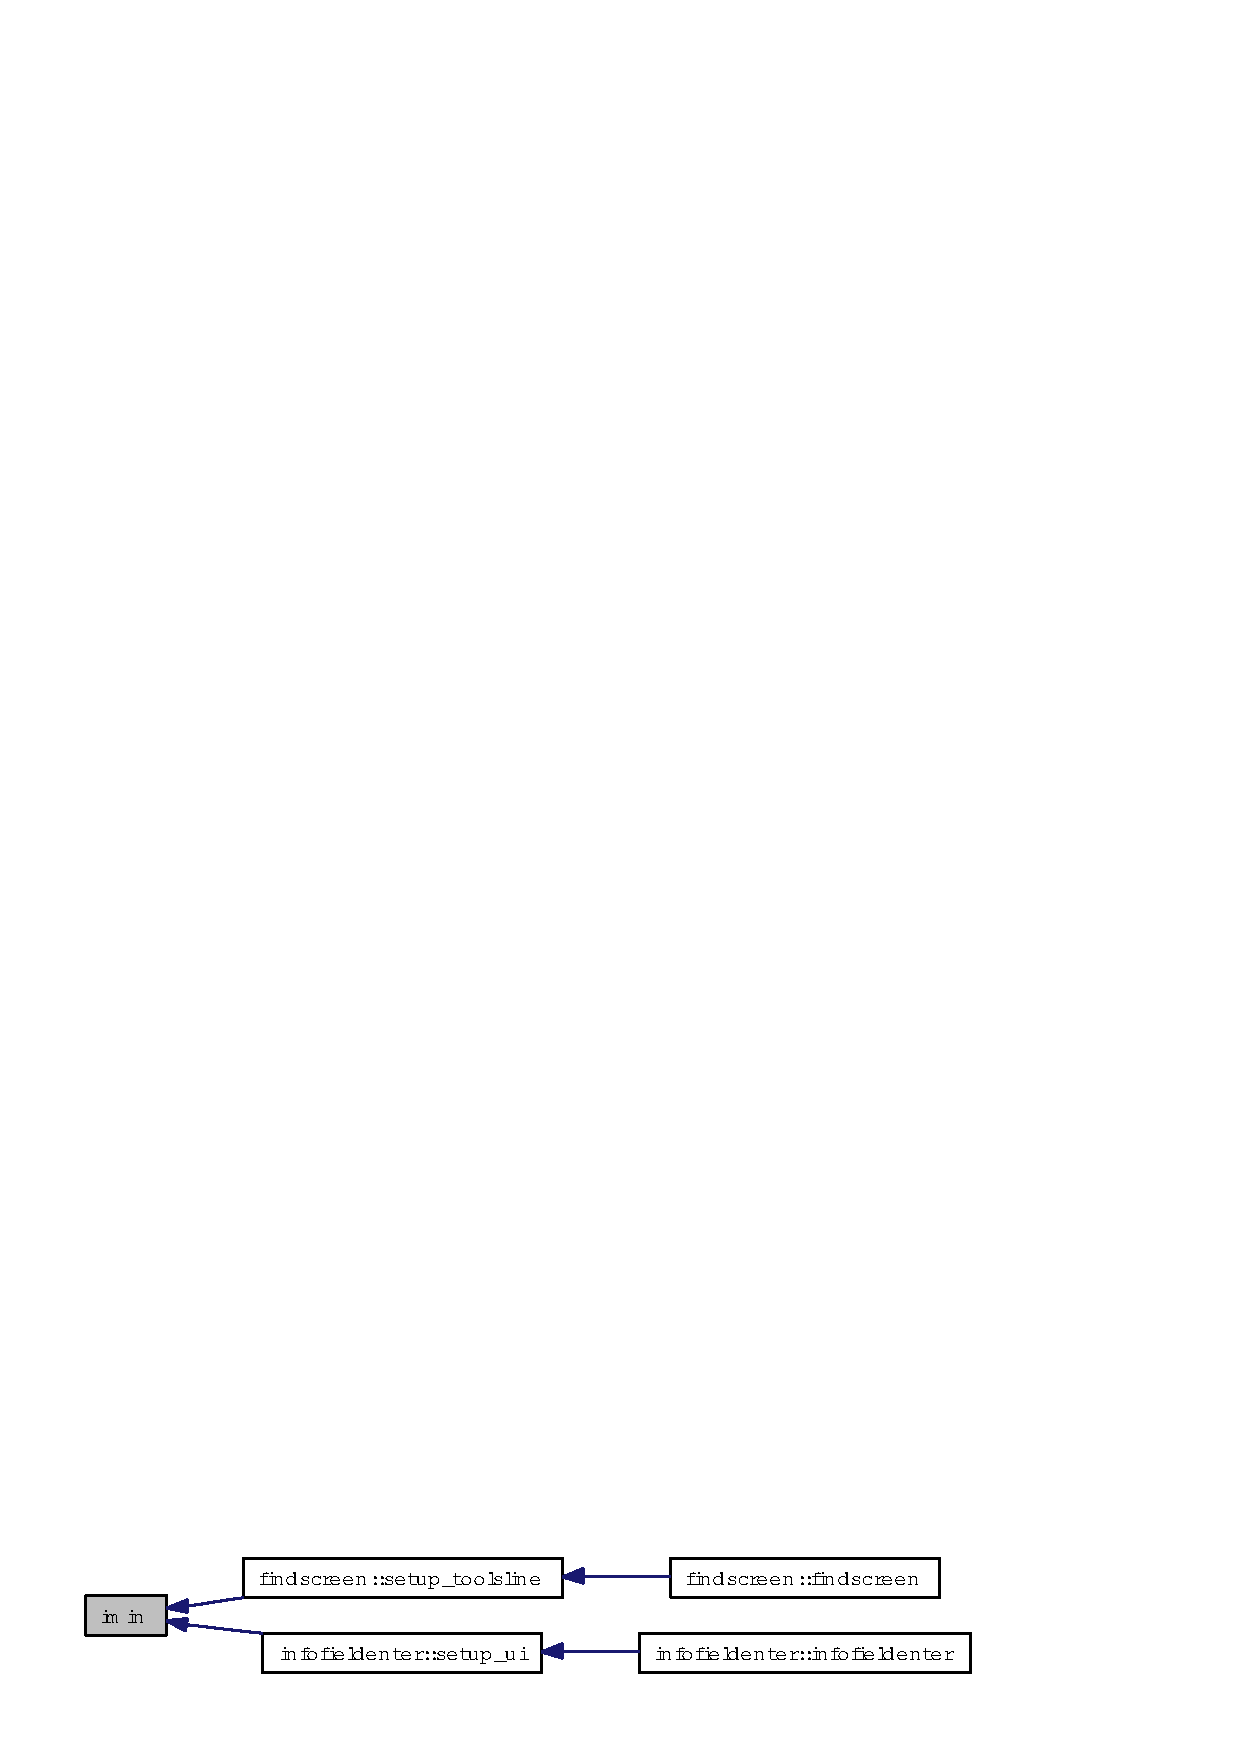
\includegraphics[width=235pt]{main_8h_6c9ac00d126f1109a583b5264a07412a_icgraph}
\end{center}
\end{figure}
\index{main.h@{main.h}!info_window@{info\_\-window}}
\index{info_window@{info\_\-window}!main.h@{main.h}}
\subsubsection{\setlength{\rightskip}{0pt plus 5cm}void info\_\-window (QString {\em i})}\label{main_8h_11a7110d2888630c2a28e17fcd3199fd}




Definition at line 50 of file main.cpp.

Referenced by editor::on\_\-showhtml\_\-clicked().\index{main.h@{main.h}!logprint@{logprint}}
\index{logprint@{logprint}!main.h@{main.h}}
\subsubsection{\setlength{\rightskip}{0pt plus 5cm}void logprint (char $\ast$ {\em lpsz\-Text},  {\em ...})}\label{main_8h_e8160c24b0b45e234c5ad305d0d31a3b}




Definition at line 12 of file main.cpp.\index{main.h@{main.h}!print_object_tree@{print\_\-object\_\-tree}}
\index{print_object_tree@{print\_\-object\_\-tree}!main.h@{main.h}}
\subsubsection{\setlength{\rightskip}{0pt plus 5cm}void print\_\-object\_\-tree (void)}\label{main_8h_8ff96661921f7c09201747e09d034951}




Definition at line 214 of file main.cpp.

References mainwindowpointer, and print\_\-object\_\-tree\_\-recurse().

Referenced by main().

Here is the call graph for this function:\begin{figure}[H]
\begin{center}
\leavevmode
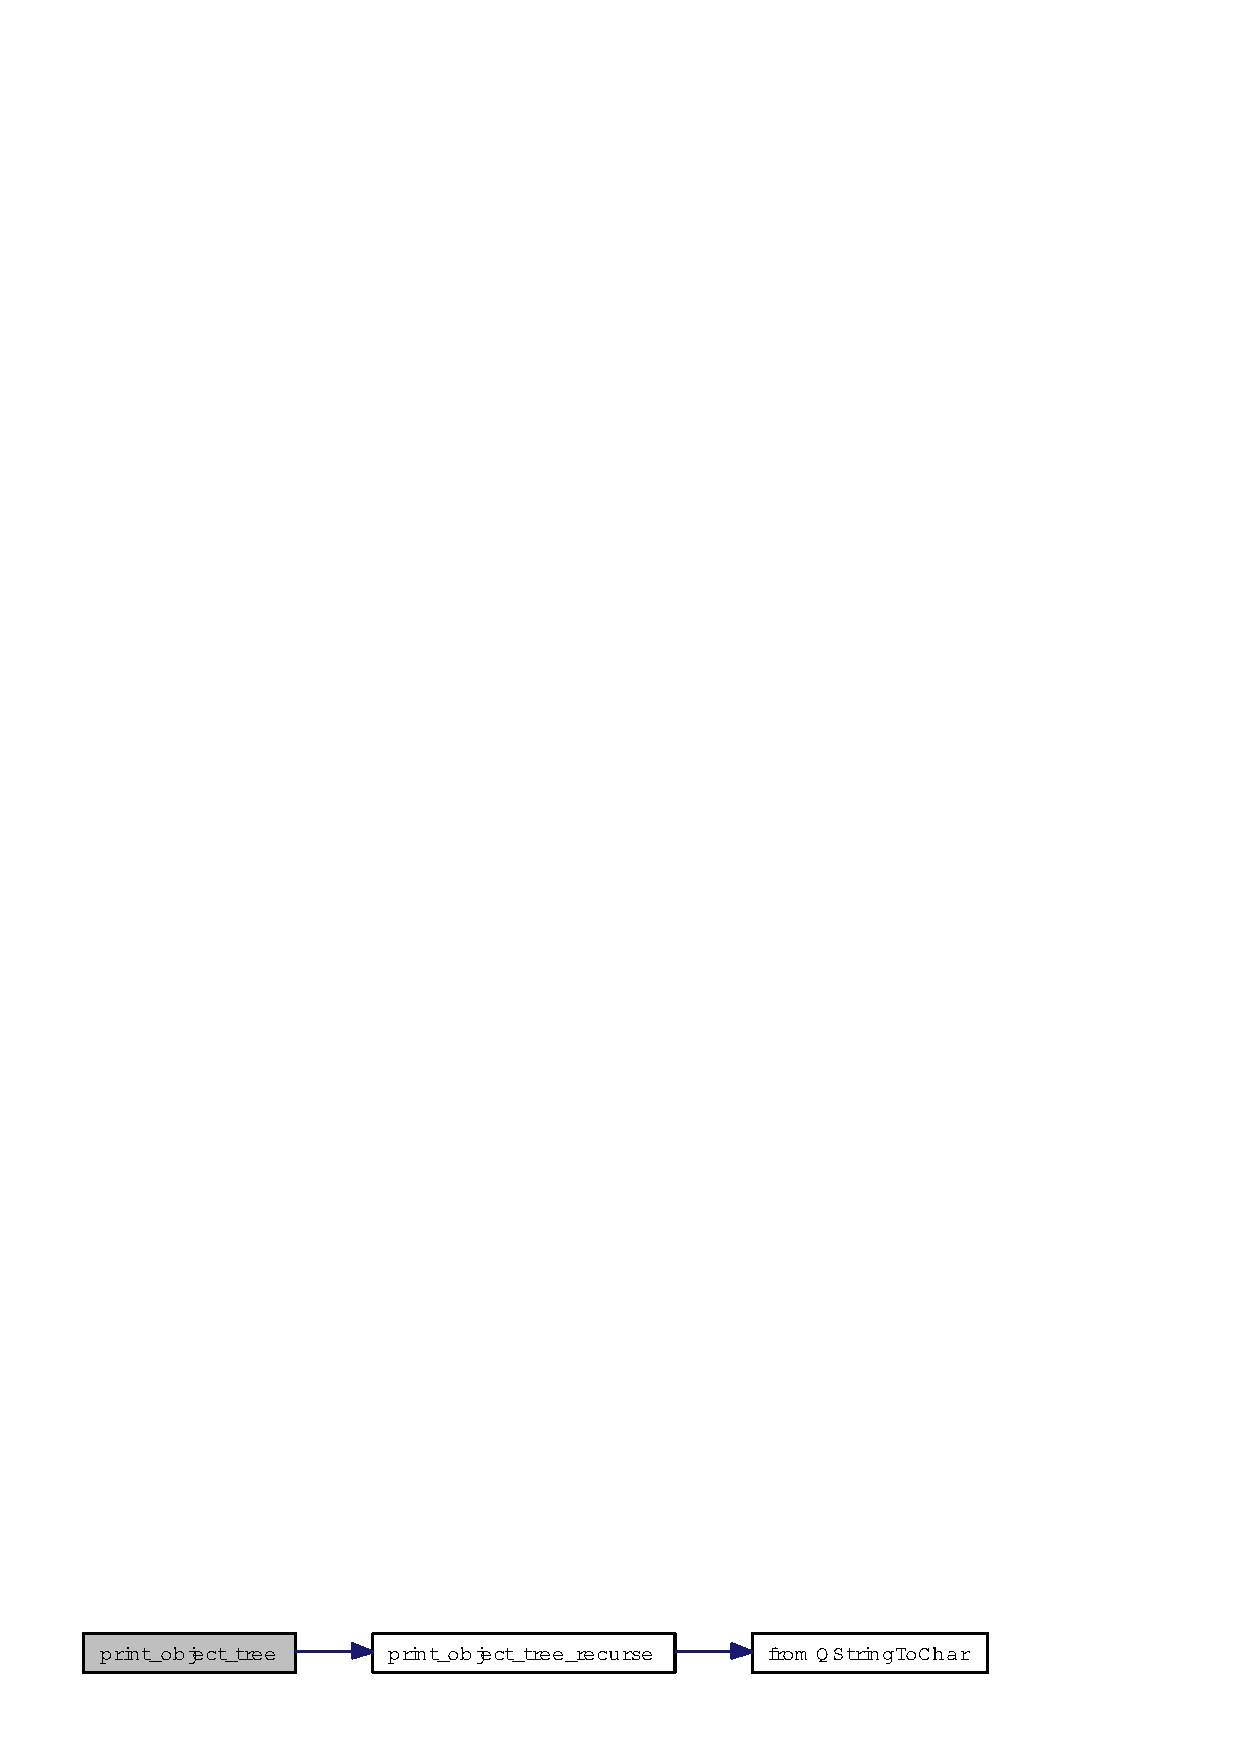
\includegraphics[width=239pt]{main_8h_8ff96661921f7c09201747e09d034951_cgraph}
\end{center}
\end{figure}


Here is the caller graph for this function:\begin{figure}[H]
\begin{center}
\leavevmode
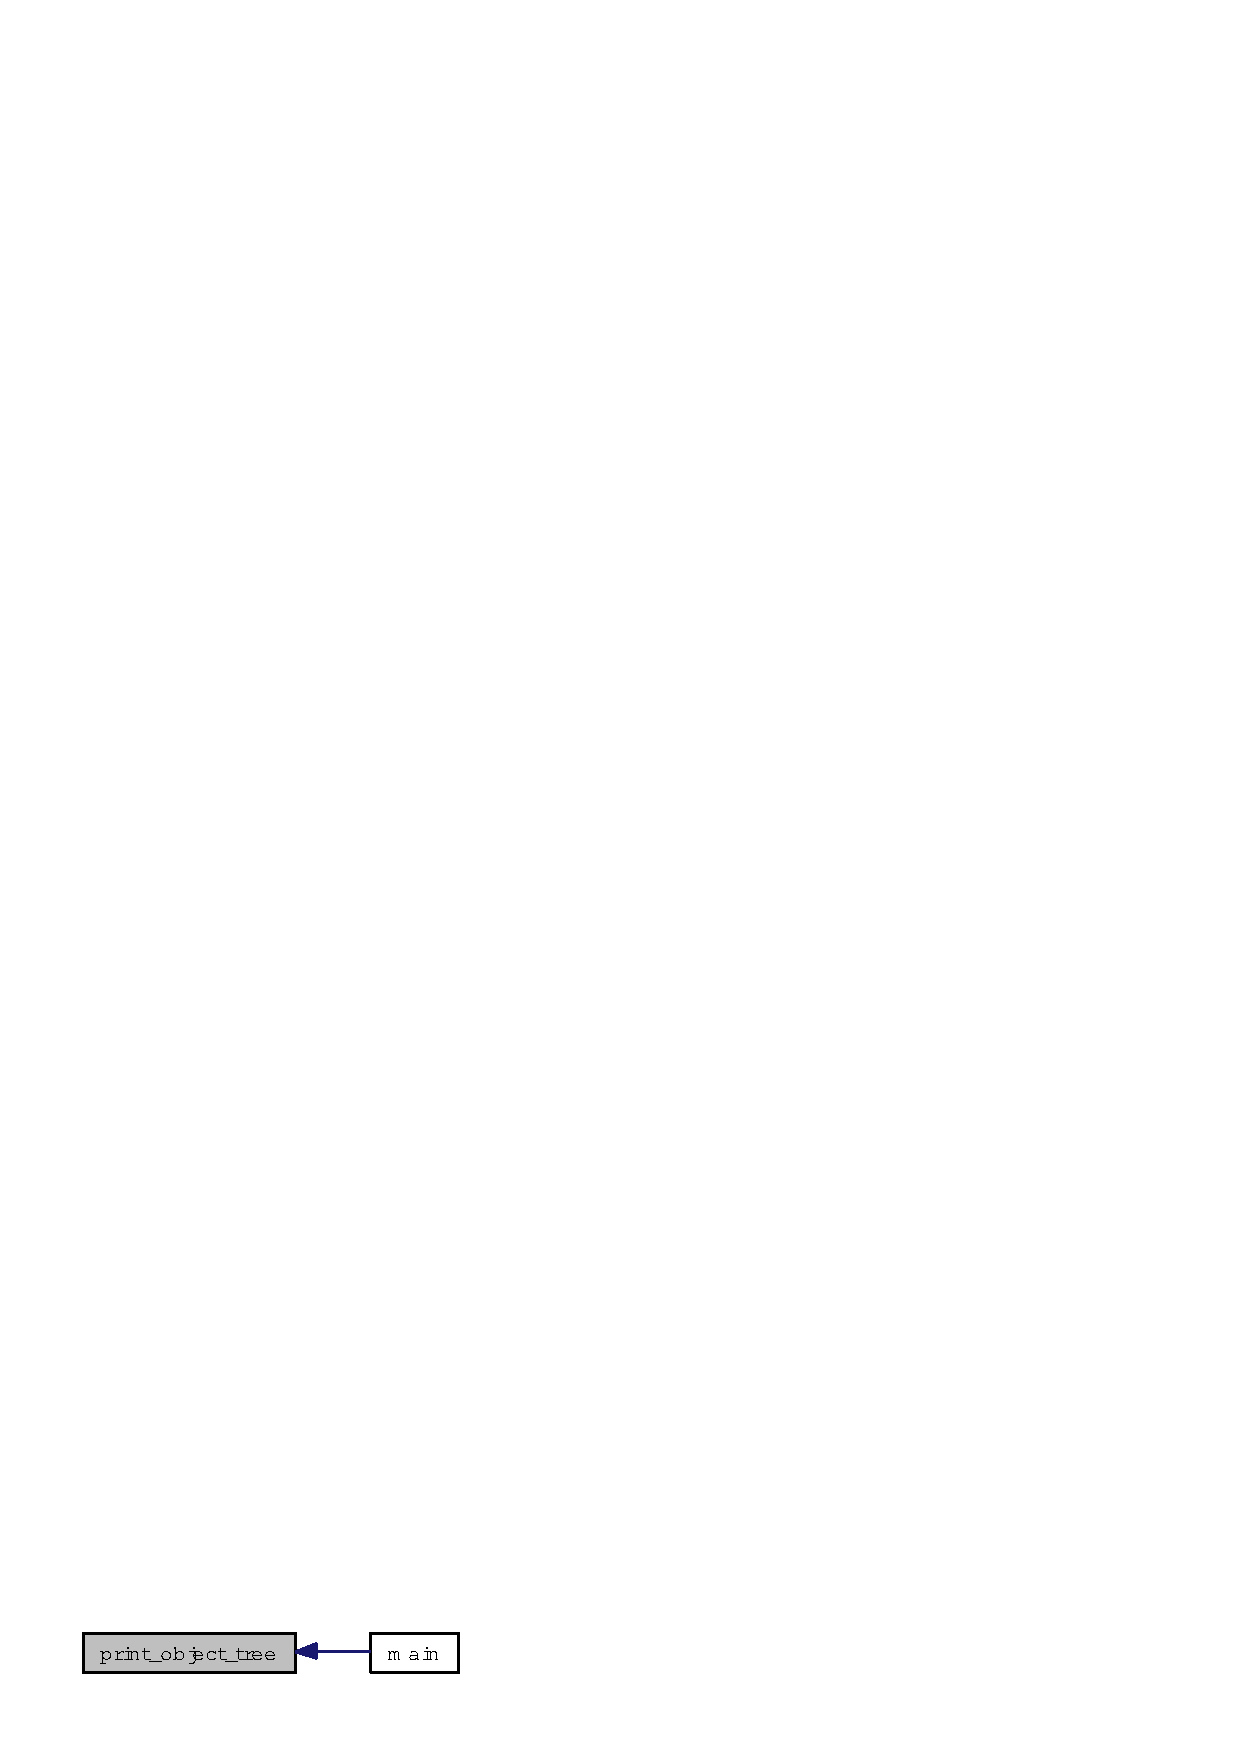
\includegraphics[width=112pt]{main_8h_8ff96661921f7c09201747e09d034951_icgraph}
\end{center}
\end{figure}
\index{main.h@{main.h}!remove_dir@{remove\_\-dir}}
\index{remove_dir@{remove\_\-dir}!main.h@{main.h}}
\subsubsection{\setlength{\rightskip}{0pt plus 5cm}void remove\_\-dir (QString {\em namedirfrom})}\label{main_8h_6ac3f8d337a3e659a3c1cdfeef1cbaf0}




Definition at line 125 of file main.cpp.

References appconfig::get\_\-lastprefixnum\_\-as\_\-line(), appconfig::get\_\-trashdir(), appconfig::inc\_\-lastprefixnum(), and mytetraconfig.

Referenced by recordtabledata::delete\_\-record().

Here is the call graph for this function:\begin{figure}[H]
\begin{center}
\leavevmode
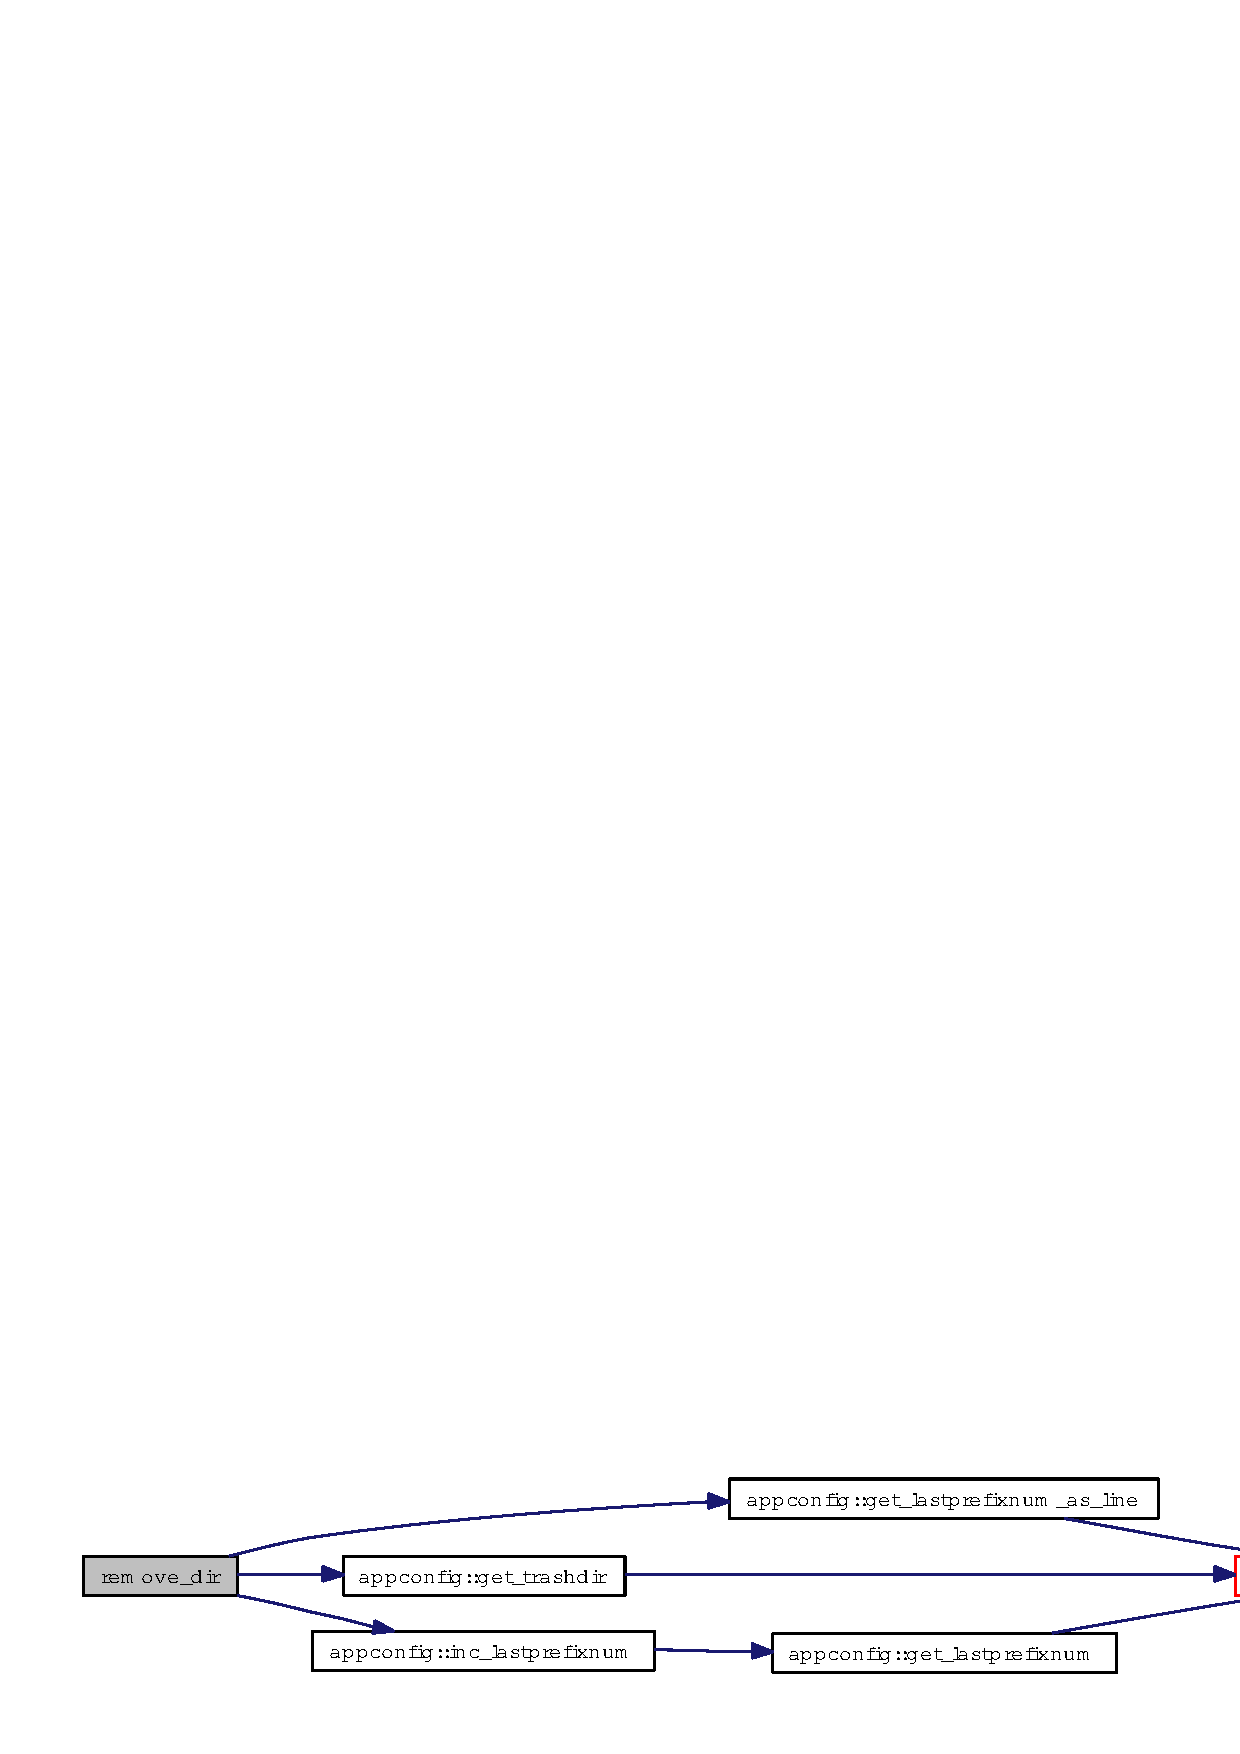
\includegraphics[width=373pt]{main_8h_6ac3f8d337a3e659a3c1cdfeef1cbaf0_cgraph}
\end{center}
\end{figure}


Here is the caller graph for this function:\begin{figure}[H]
\begin{center}
\leavevmode
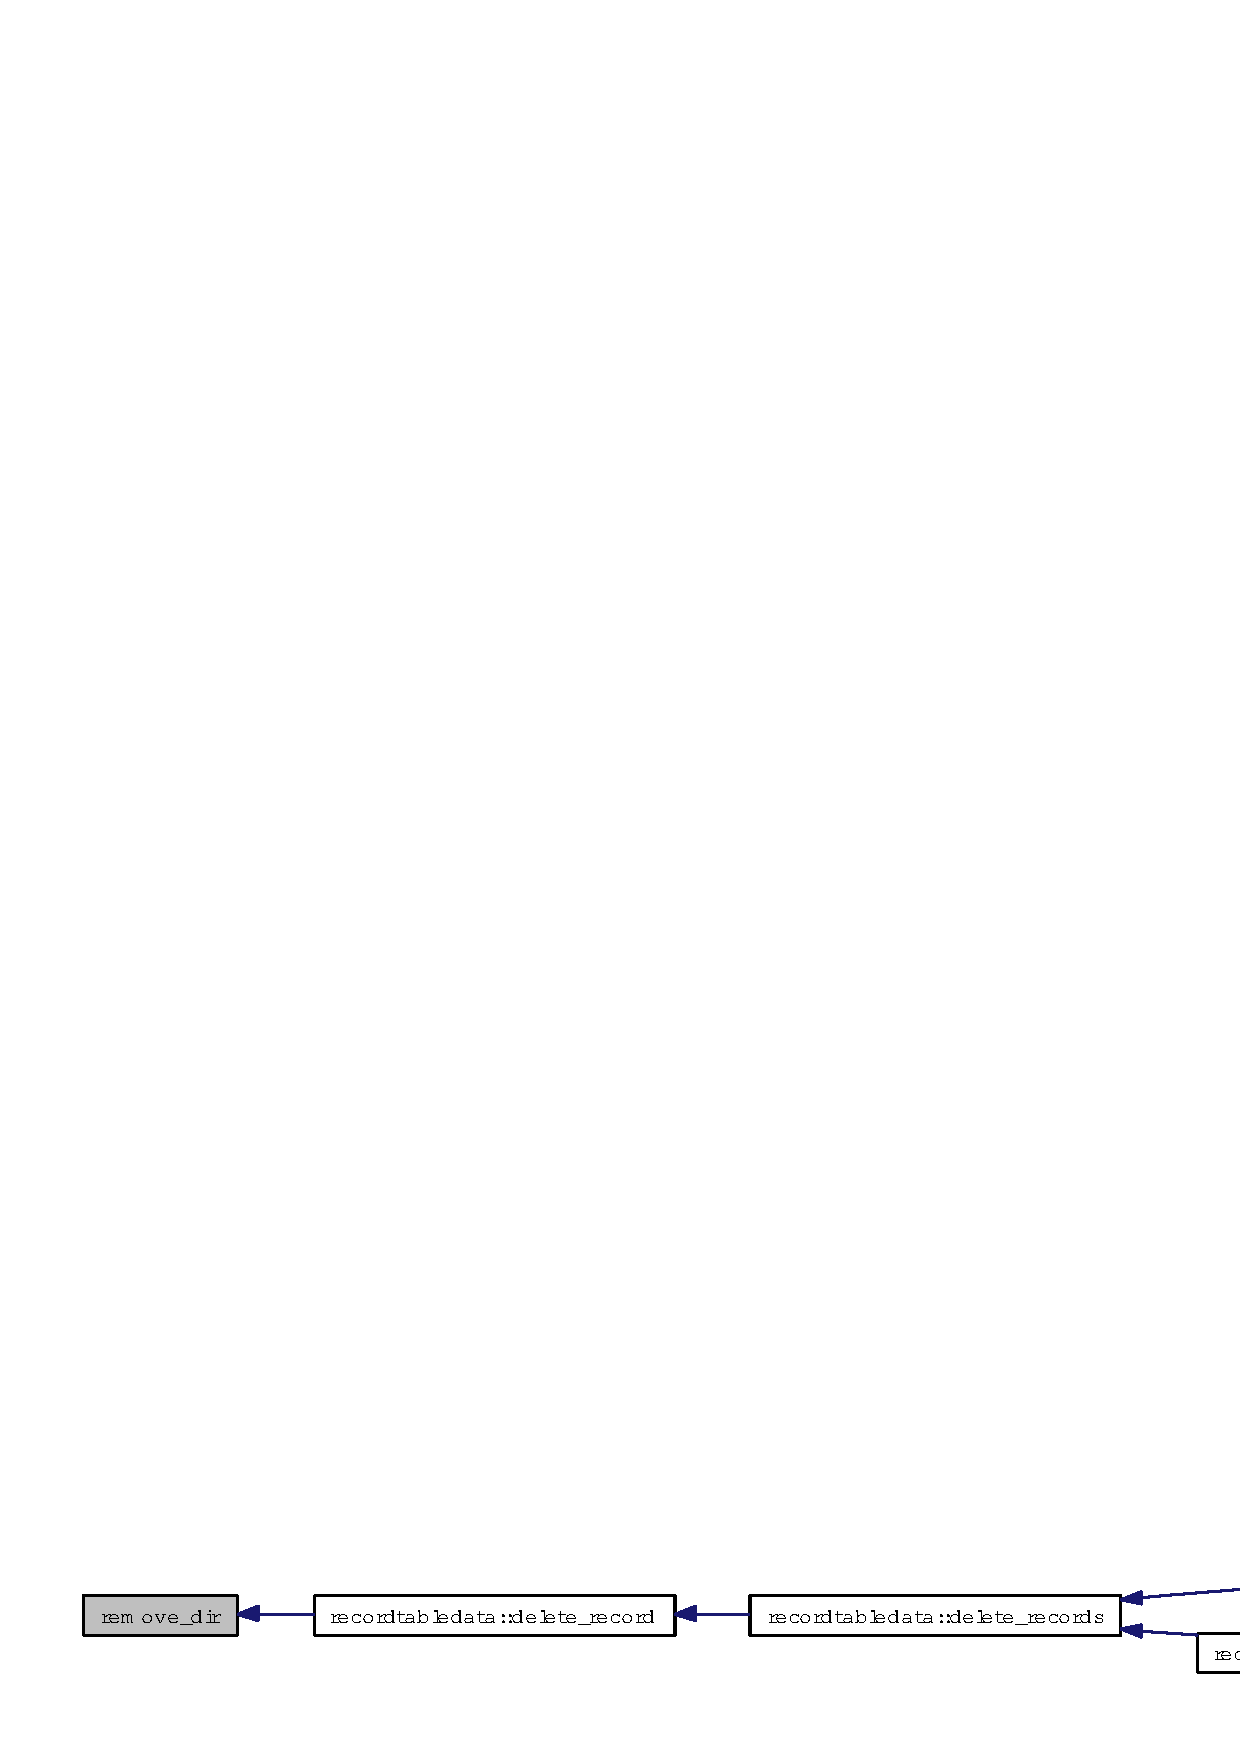
\includegraphics[width=384pt]{main_8h_6ac3f8d337a3e659a3c1cdfeef1cbaf0_icgraph}
\end{center}
\end{figure}
\index{main.h@{main.h}!xmlnode_to_string@{xmlnode\_\-to\_\-string}}
\index{xmlnode_to_string@{xmlnode\_\-to\_\-string}!main.h@{main.h}}
\subsubsection{\setlength{\rightskip}{0pt plus 5cm}QString xmlnode\_\-to\_\-string (QDom\-Node {\em xmldata})}\label{main_8h_dbcd54017c14dc5f88b7ff9e17a87706}




Definition at line 73 of file main.cpp.